\documentclass[spanish,a4paper,14pt,oneside]{extreport}

%%%%%%%%%%%%%%%%%%%%%%%%%%%%%%%%%%%%%%%%%%%%%%%%%%%%%%%%%%%%%%%%%%%%%%%%%%%%%%%
\usepackage[dvips]{graphicx}
\usepackage[dvips]{epsfig}
\usepackage[utf8]{inputenc}
\usepackage[spanish]{babel}
\usepackage{alltt}
\usepackage{algorithm}
\usepackage{algorithmic}
\usepackage{multirow}
\usepackage[top=2cm, bottom=2cm, left=2cm, right=2cm]{geometry}
\usepackage[usenames]{xcolor}
\usepackage{wrapfig}
\usepackage{caption}
\usepackage[bookmarks]{hyperref}
\usepackage{listings}
\usepackage[gen]{eurosym}


\lstset{
  frame=single,
  breaklines=true,
  postbreak=\raisebox{0ex}[0ex][0ex]{\ensuremath{\color{red}\hookrightarrow\space}}
}
%%%%%%%%%%%%%%%%%%%%%%%%%%%%%%%%%%%%%%%%%%%%%%%%%%%%%%%%%%%%%%%%%%%%%%%%%%%%%%%

\newcommand{\SONY}{{\sc Sony}}
\newcommand{\MICROSOFT}{{\sc Microsoft}}
\newcommand{\GCC}{\textsf{\textsc{G}CC}}
\newcommand{\INTEL}{\textsf{\textsc{I}ntel}}

%%% Traducimos el pseudocodigo
\renewcommand{\algorithmicwhile}{\textbf{mientras}}
\renewcommand{\algorithmicend}{\textbf{fin}}
\renewcommand{\algorithmicdo}{\textbf{hacer}}
\renewcommand{\algorithmicif}{\textbf{si}}
\renewcommand{\algorithmicthen}{\textbf{entonces}}
\renewcommand{\algorithmicrepeat}{\textbf{repetir}}
\renewcommand{\algorithmicuntil}{\textbf{hasta que}}
\renewcommand{\algorithmicelse}{\textbf{en otro caso}}
\renewcommand{\algorithmicfor}{\textbf{para}}

%\newcommand{\RETURN}{\textbf{retornar} }
\newcommand{\RET}{\STATE \textbf{retornar} }
\newcommand{\TO}{\textbf{hasta} }
\newcommand{\AND}{\textbf{y} }
\newcommand{\OR}{\textbf{o} }

%%%%%%%%%%%%%%%%% Creamos un entorno para listar código fuente %%%%%%%%%%%%%%%
\newenvironment{sourcecode}
{\begin{list}{}{\setlength{\leftmargin}{1em}}\item\scriptsize\bfseries}
{\end{list}}

\newenvironment{littlesourcecode}
{\begin{list}{}{\setlength{\leftmargin}{1em}}\item\tiny\bfseries}
{\end{list}}

\newenvironment{summary}
{\par\noindent\begin{center}\textbf{Abstract}\end{center}\begin{itshape}\par\noindent}
{\end{itshape}}

\newenvironment{keywords}
{\begin{list}{}{\setlength{\leftmargin}{1em}}\item[\hskip\labelsep \bfseries Keywords:]}
{\end{list}}

\newenvironment{palabrasClave}
{\begin{list}{}{\setlength{\leftmargin}{1em}}\item[\hskip\labelsep \bfseries Palabras clave:]}
{\end{list}}


%%%%%%%%%%%%%%%%%%%%%%%%%%%%%%%%%%%%%%%%%%%%%%%%%%%%%%%%%%%%%%%%%%%%%%%%%%%%%%%
% Format
%%%%%%%%%%%%%%%%%%%%%%%%%%%%%%%%%%%%%%%%%%%%%%%%%%%%%%%%%%%%%%%%%%%%%%%%%%%%%%%
%\usepackage{showframe}
%\marginparwidth 0mm
%%\topmargin -4 mm
%\topmargin -21 mm
%\headheight 10 mm
%\headsep 10 mm

%\textheight 229 mm
%\textheight 246 mm

%\oddsidemargin -5.4 mm
%\evensidemargin -5.4 mm
%\oddsidemargin 5 mm
%\evensidemargin 5 mm

%\oddsidemargin -3 mm
%\evensidemargin -3 mm

%\textwidth 17 cm
%\textwidth 15 cm
%\columnsep 10 mm

\input{amssym.def}

%%%%%%%%%%%%%%%%%%%%%%%%%%%%%%%%%%%%%%%%%%%%%%%%%%%%%%%%%%%%%%%%%%%%%%%%%%%%%%%

\begin{document}

%%%%%%%%%%%%%%%%%%%%%%%%%%%%%%%%%%%%%%%%%%%%%%%%%%%%%%%%%%%%%%%%%%%%%%%%%%%%%%%
% First Page
%%%%%%%%%%%%%%%%%%%%%%%%%%%%%%%%%%%%%%%%%%%%%%%%%%%%%%%%%%%%%%%%%%%%%%%%%%%%%%%

\pagestyle{empty}
\thispagestyle{empty}


\newcommand{\HRule}{\rule{\linewidth}{1mm}}
\setlength{\parindent}{0mm}
\setlength{\parskip}{10pt}

\vspace*{\stretch{0.5}}

\begin{center}
\includegraphics[scale=0.8]{images/logo_vertical}\\[10mm]
{\Huge Trabajo de Fin de Grado}
\end{center}

\HRule
\begin{flushright}
        {\Huge Visión artificial aplicada a la robótica} \\[2.5mm]
        {\Large \textit{Artificial vision applied to robotics} .} \\[5mm]
        {\Large Miguel Ángel Delgado Hernández} \\[5mm]


\end{flushright}
\HRule
\vspace*{\stretch{2}}
\begin{center}
  \Large La Laguna, \today
\end{center}

\setlength{\parindent}{5mm}

%%%%%%%%%%%%%%%%%%%%%%%%%%%%%%%%%%%%%%%%%%%%%%%%%%%%%%%%%%%%%%%%%%%%%%%%%%%%%%%
% Signature page (add the official stamp)
%%%%%%%%%%%%%%%%%%%%%%%%%%%%%%%%%%%%%%%%%%%%%%%%%%%%%%%%%%%%%%%%%%%%%%%%%%%%%%%
\newpage
%\cleardoublepage
\thispagestyle{empty}

D. {\bf Jonay Tomás Toledo Carrillo}, con N.I.F. 78.698.554-Y
profesor
Contratado Doctor de Universidad
adscrito al Departamento
de Ing. Informática y de Sistemas
de la Universidad de La Laguna, como tutor

\bigskip
\bigskip
{\bf C E R T I F I C A}

\bigskip
\bigskip
\bigskip
Que la presente memoria titulada:

\bigskip
``{\it Visión artificial aplicada a la robótica.}''

\bigskip
\bigskip
\bigskip

\noindent ha sido realizada bajo su dirección por D. {\bf Miguel Ángel Delgado Hernández},
con N.I.F. 54.112.876-V.

\bigskip
\bigskip

Y para que así conste, en cumplimiento de la legislación vigente y a los efectos
oportunos firman la presente en La Laguna a \today

%\cleardoublepage
\newpage
%%%%%%%%%%%%%%%%%%%%%%%%%%%%%%%%%%%%%%%%%%%%%%%%%%%%%%%%%%%%%%%%%%%%%%%%%%%%%%%
\thispagestyle{empty}

{ \flushright

\begin{LARGE}
Agradecimientos
\end{LARGE}

\hspace{3mm}

\begin{large}


\hspace{3mm}
En primer lugar me gustaría agradecer a mi tutor académico, Jonay Tomás Toledo
Carrillo, porque sin su inconmensurable ayuda no podría haber desarrollado este
proyecto hasta el final, siempre atento y abierto a resolver dudas.

\hspace{3mm}
En segundo lugar me gustaría agradecer a mis dos compañeros y amigos, Andrés
Cidoncha Carballo y Fabián Díaz Lorenzo, porque ellos más que nadie conocen
tanto los buenos como los momentos más difíciles, y juntos nos hemos apoyado
para aprender de los conocimientos de los tres.

\hspace{3mm}
Finalmente agradecer al resto de familiares y demás amigos que también me han
apoyado en todo momento. 

\hspace{3mm}
Muchas gracias a todos.


\end{large}

}

%%%%%%%%%%%%%%%%%%%%%%%%%%%%%%%%%%%%%%%%%%%%%%%%%%%%%%%%%%%%%%%%%%%%%%%%%%%%%%%%%
\newpage

\begin{huge}
Licencia
\end{huge}

\begin{center}
\includegraphics[scale=1.5]{images/by-nc-sa_88x31}\\[10mm]
{\Large \copyright~Esta obra está bajo una licencia de Creative Commons Reconocimiento-NoComercial-CompartirIgual 4.0 Internacional.
}
\end{center}

%%%%%%%%%%%%%%%%%%%%%%%%%%%%%%%%%%%%%%%%%%%%%%%%%%%%%%%%%%%%%%%%%%%%%%%%%%%%%%%
\newpage  %\cleardoublepage
\begin{abstract}
{\em

El objetivo de este trabajo ha sido la reconstrucción de mapas tridimensionales
del entorno a partir de sistemas estereoscópicos de dos cámaras para la
localización de un robot en el mismo.

\bigskip
Las cámaras son uno de los sensores que pueden dar una información más rica del
entorno para un robot. Con el uso de dos cámaras se puede conocer no solo la
imagen en color sino también la distancia a los objetos, haciendo de la
información visual, información espacial. Esta información espacial puede ser
integrada para la reconstrucción de mapas en 3D.

\bigskip
Este sistema estereoscópico ha sido probado sobre el proyecto Perenquén, un
robot autónomo realizado por el Grupo de Robótica de la Universidad de La
Laguna, para la reconstrucción de los mapas en exteriores, donde los sensores
actuales del robot se ven muy limitados.
}

\begin{palabrasClave}
visión estereoscópica, reconstrucción 3D, localización, odometría, ros
\end{palabrasClave}

\end{abstract}
%%%%%%%%%%%%%%%%%%%%%%%%%%%%%%%%%%%%%%%%%%%%%%%%%%%%%%%%%%%%%%%%%%%%%%%%%%%%%%%

%%%%%%%%%%%%%%%%%%%%%%%%%%%%%%%%%%%%%%%%%%%%%%%%%%%%%%%%%%%%%%%%%%%%%%%%%%%%%%%
\newpage  %\cleardoublepage
\begin{summary}
{\em

The purpose of this project has been 3D mapping of environment using a
stereostopic vision system by two cameras for robot localization in this map.

\bigskip
Vision systems are one of the best sensors to get valuable information about
environment. The use of a stereo camera is the most widespread usage due to it's
low price and the good results that can be achieved. Through stereo camera
approach is possible to recognize color image further distance to objects,
meaning visual information can turn into spatial information. The spatial
information can be integrated to get 3D mapping.

\bigskip
This stereoscopic vision system has been tested on Perenquén project, an
autonomous robot made by Robotics Group of the University of La Laguna, for 3D
mapping in extenral spaces, where current sensors of teh rebot are very limited.
}

\begin{keywords}
stereo vision, 3D mapping, localization, odometry, ros
\end{keywords}

\end{summary}
%%%%%%%%%%%%%%%%%%%%%%%%%%%%%%%%%%%%%%%%%%%%%%%%%%%%%%%%%%%%%%%%%%%%%%%%%%%%%%%

%%%%%%%%%%%%%%%%%%%%%%%%%%%%%%%%%%%%%%%%%%%%%%%%%%%%%%%%%%%%%%%%%%%%%%%%%%%%%%%
\newpage{\pagestyle{empty}}
\thispagestyle{empty}

%%%%%%%%%%%%%%%%%%%%%%%%%%%%%%%%%%%%%%%%%%%%%%%%%%%%%%%%%%%%%%%%%%%%%%%%%%%%%%%


\pagestyle{myheadings} %my head defined by markboth or markright
% No funciona bien \markboth sin "twoside" en \documentclass, pero al
% ponerlo se dan un montón de errores de underfull \vbox, con lo que no se
% ha puesto.
\markboth{Miguel Ángel Delgado Hernández}{Visión artificial aplicada a la robótica}

%%%%%%%%%%%%%%%%%%%%%%%%%%%%%%%%%%%%%%%%%%%%%%%%%%%%%%%%%%%%%%%%%%%%%%%%%%%%%%%
%Numeracion en romanos
\renewcommand{\thepage}{\roman{page}}
\setcounter{page}{1}

%%%%%%%%%%%%%%%%%%%%%%%%%%%%%%%%%%%%%%%%%%%%%%%%%%%%%%%%%%%%%%%%%%%%%%%%%%%%%%%

\tableofcontents

%%%%%%%%%%%%%%%%%%%%%%%%%%%%%%%%%%%%%%%%%%%%%%%%%%%%%%%%%%%%%%%%%%%%%%%%%%%%%%%
\newpage{\pagestyle{empty}}

\listoffigures

%%%%%%%%%%%%%%%%%%%%%%%%%%%%%%%%%%%%%%%%%%%%%%%%%%%%%%%%%%%%%%%%%%%%%%%%%%%%%%%
\newpage{\pagestyle{empty}}

\listoftables

%%%%%%%%%%%%%%%%%%%%%%%%%%%%%%%%%%%%%%%%%%%%%%%%%%%%%%%%%%%%%%%%%%%%%%%%%%%%%%%
\newpage{\pagestyle{empty}}

%%%%%%%%%%%%%%%%%%%%%%%%%%%%%%%%%%%%%%%%%%%%%%%%%%%%%%%%%%%%%%%%%%%%%%%%%%%%%%%
%Numeracion a partir del capitulo I
\renewcommand{\thepage}{\arabic{page}}
\setcounter{page}{1}


\chapter{Introducción}
\label{chapter:introduccion}

%%%%%%%%%%%%%%%%%%%%%%%%%%%%%%%%%%%%%%%%%%%%%%%%%%%%%%%%%%%%%%%%%%%%%%%%%%%%%
% Chapter 1: Introducción
%%%%%%%%%%%%%%%%%%%%%%%%%%%%%%%%%%%%%%%%%%%%%%%%%%%%%%%%%%%%%%%%%%%%%%%%%%%%%%%
% \textcolor{red}{text}
%---------------------------------------------------------------------------------
\section{Contexto}
\label{1:sec:1}

Puntos clave: robots, sistemas guiados, camaras estereoscopicas, deteccion de
obstaculos

Las cámaras son uno de los sensores que pueden dar una información mas
rica del entorno para un robot. En este proyecto se plantea la utilización de
cámaras y de sistemas estereoscópicos de dos cámaras para la detección de
obstáculos y su posterior esquiva.

%---------------------------------------------------------------------------------
\section{Objetivo}
\label{1:sec:2}

El tema central de este proyecto es muy ambicioso, de este modo, es necesario
poder realizar una distinción entre el objetivo principal y los objetivos
específicos que lo rodean.

\subsection{Objetivo general}

\textcolor{red}{¿Detección y esquiva o reconstrucción del mapa?}

El objetivo principal de este Trabajo de Fin de Grado es poder integrar el uso
de un sistema estereoscópico de dos cámaras en un robot, para la detección y
posteriormente esquiva de los obstáculos que se encuentren.

\subsection{Objetivos específicos}

Los objetivos específicos que componen el proyecto son:
% \newline
\begin{itemize}
\item Uso de una cámara comercial de entretenimiento en un proyecto de
investigación.
\item Reconstrucción de un mapa tridimensional a partir de las imágenes
recogidas por las cámaras.
\item Integración de cámaras estereoscópicas junto a otros sistemas de detección
de obstáculos.
\end{itemize}

%---------------------------------------------------------------------------------
% \section{Sección Tres}
% \label{1:sec:3}
% \begin{itemize}
%   \item Item 1
%   \item Item 2
%   \item Item 3
% \end{itemize}
% Bla, bla, bla

%---------------------------------------------------------------------------------
% \section{Sección Cuatro}
%   \label{1:sec:4}
%
% Bla, bla, bla

%------------------------------------------------------------------------------
% \begin{figure}[!th]
% \begin{center}
% \includegraphics[width=0.5\textwidth]{images/arbolbinario.eps}
% \caption{Ejemplo}
% \label{fig:ArbolBinario}
% \end{center}
% \end{figure}
%------------------------------------------------------------------------------


%%%%%%%%%%%%%%%%%%%%%%%%%%%%%%%%%%%%%%%%%%%%%%%%%%%%%%%%%%%%%%%%%%%%%%%%%%%%%%%

\chapter{Conceptos}
\label{chapter:conceptos}

%%%%%%%%%%%%%%%%%%%%%%%%%%%%%%%%%%%%%%%%%%%%%%%%%%%%%%%%%%%%%%%%%%%%%%%%%%%%%%%%
% Chapter 2: Conceptos
%%%%%%%%%%%%%%%%%%%%%%%%%%%%%%%%%%%%%%%%%%%%%%%%%%%%%%%%%%%%%%%%%%%%%%%%%%%%%%%%

%+++++++++++++++++++++++++++++++++++++++++++++++++++++++++++++++++++++++++++++++
En este capítulo se abordarán todos aquellos conceptos teóricos que han surgido
a lo largo del proyecto y son necesarios para entender correctamente la línea
del trabajo.


%+++++++++++++++++++++++++++++++++++++++++++++++++++++++++++++++++++++++++++++++
\section{Visión artificial}
\label{2:sec:1}
% https://campusvirtual.ull.es/1516/course/view.php?id=202
% https://es.wikipedia.org/wiki/Visi%C3%B3n_artificial
% https://en.wikipedia.org/wiki/Computer_vision
% J. GONZÁLEZ JIMÉNEZ, "Visión Por Computador", Editorial Paraninfo. 2000

La visión artificial por computador, es la disciplina científica que se basa en
la adquisición, procesamiento y análisis de las imágenes que se toman del mundo
real, con el objetivo de obtener información relevante acerca de ellas:
detección de objetos, seguimiento del movimiento, reconocimiento de eventos,
etc. Un ejemplo que podemos ver en nuestro día a día, es la detección de caras
en una escena capturada por una cámara digital o smartphone, mediante el uso de
téncicas de reconocimiento de patrones.

Al igual que sucede en otras áreas de la inteligencia artificial, la visión
artificial tiene como objetivo principal obtener la información explícita y el
significado de la realidad de la misma manera que lo haría un ser biológico.

El avance progresivo del hardware con nuevos procesadores digitales de señales
(DSP) y unidades de procesamiento gráfico (GPU), junto con nuevas tecnologías y planteamientos de cómputo como la computación paralela, ha permitido que en los
últimos años se haya podido implementar nuevos algortimos más rápidos y
eficientes, necesarios para ser utilizados en ámbitos críticos, como sistemas
en tiempo real.

%--------------------------------------
\subsection{Objetivos}

\textcolor{red}{Lorem ipsum dolor sit amet, consectetur adipisicing elit, sed do
 eiusmod tempor incididunt ut labore et dolore magna aliqua. Ut enim ad minim 
 veniam, quis nostrud exercitation ullamco laboris nisi ut aliquip ex ea commodo 
 consequat. Duis aute irure dolor in reprehenderit in voluptate velit esse cillum
 dolore eu fugiat nulla pariatur. Excepteur sint occaecat cupidatat non proident,
 sunt in culpa qui officia deserunt mollit anim id est laborum.}

\textcolor{red}{Lorem ipsum dolor sit amet, consectetur adipisicing elit, sed do
 eiusmod tempor incididunt ut labore et dolore magna aliqua. Ut enim ad minim 
 veniam, quis nostrud exercitation ullamco laboris nisi ut aliquip ex ea commodo 
 consequat. Duis aute irure dolor in reprehenderit in voluptate velit esse cillum
 dolore eu fugiat nulla pariatur. Excepteur sint occaecat cupidatat non proident,
 sunt in culpa qui officia deserunt mollit anim id est laborum.}

%--------------------------------------
\subsection{Dificultades}
La capacidad visual es uno pilares de la inteligencia humana. Su implementación
en la rotótica supone también un importante avance en la inteligencia artificial.
Sin embargo, mientras que la percepción visual es algo innato y cotidiano para
nosotros, la visión artificial es muy compleja y conlleva muchas dificultades.
Entre las principales dificultades, destacan:

\begin{itemize}
  \item \textbf{Mundo tridimensional:} mientras que las imágenes que se obtienen
  con una cámara son bidimensionales, el mundo que nos rodea no. Es necesario 
  realizar las transformaciones correspondientes para obtener valores correctos.
  \item \textbf{Zonas de interés:} se necesita extraer elementos de información 
  sutiles en imágenes complejas, por lo que entre tanta información es necesario
  reconocer formas, colores, etc.
  \item \textbf{Carácter dinámico de las escenas:} el mundo está vivo, por lo
  que en las imágenes que se toman muchos elementos están en movimiento. Por 
  otro lado, otros factores como luminosidad, contraste, foco... pueden marcar
  una importante diferencia, y por desgracia, estos factores son variables, no
  se pueden controlar.
\end{itemize}

%--------------------------------------
% \subsection{Reconocimiento}

% Detección de objetos

%--------------------------------------
% \subsection{Motion Analysis}

% Video grabación de imágenes de seguridad

%--------------------------------------
% \subsection{Reconstrucción}


%+++++++++++++++++++++++++++++++++++++++++++++++++++++++++++++++++++++++++++++++
\section{Visión estéreo}
\label{2:sec:2}
% http://vision.deis.unibo.it/~smatt/Seminars/StereoVision.pdf
% http://www.cesfelipesegundo.com/revista/articulos2011/Guerrero,%20J.M.pdf

La visión estereoscópica o visión estéreo, es la técnica capaz de extraer
información tridimensional (profundidad) a partir de la posición relativa de un
objeto en imágenes bidimensionales al ser observado desde distintos ángulo por
dos o más cámaras separadas a una cierta distancia.

%--------------------------------------
\subsection{Adquisición}

Usando dos cámaras, el procedimiento a seguir para la adquisición del entorno es
capturar dos imágenes de una misma escena, desde dos cámaras separadas
ligeramente. De esta forma, las imágenes obtenidas, también tendrán un pequeño 
desplazamiento entre sí.

De manera más formal, se obtiene que para cada imagen capturada por las
cámaras, un objeto está en puntos diferentes del plano. Esta triangulazión
entre el punto P y Q y el origen de referencia, provocan una sensación de
profundidad. Mediante el sistema tradicional de una sola cámara, este punto
estaría en las mismas coordenadas.

\begin{figure}[!th]
  \begin{center}
    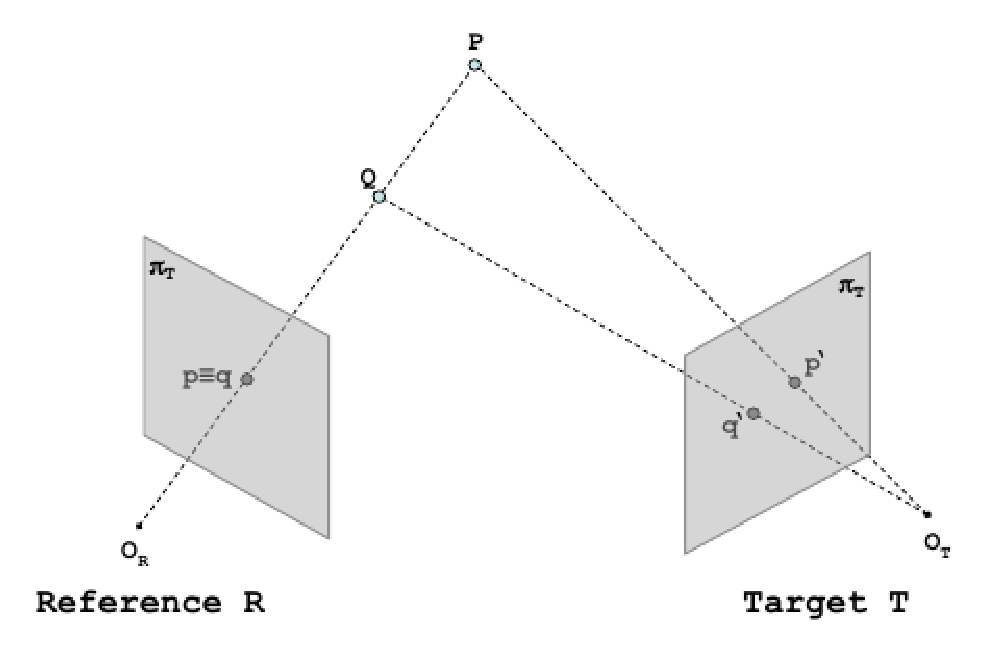
\includegraphics[width=0.7\textwidth]{images/cap2/VisionEstereo.eps}
    \caption{Diferencias entre una y dos cámaras}
    \label{fig:VisionEstereo}
  \end{center}
\end{figure}

Con estos datos, se pueden poner en correspondencia cada punto de ambas
imágenes, para obtener una imagen de disparidad (más información en la sección 
2.2.4).

%--------------------------------------
\subsection{Geometría de las cámaras}
% https://en.wikipedia.org/wiki/Parallax
% http://www.cesfelipesegundo.com/revista/articulos2011/Guerrero,%20J.M.pdf
En función de la posición relativa de las cámaras entre sí, se pueden apreciar
dos métodos principales:

\begin{itemize}
  \item \textbf{Visión paralela:} las cámaras están paralelas entre sí y están
  separadas por una línea horizonal (línea base). El objetivo que visualiza
  cada cámara es perpendicular respecto a la línea base, mientras que las
  líneas de correspondencia que unen los puntos de una imagen respecto a la otra
  son horizontales.

  \begin{minipage}{\linewidth}
      \centering
      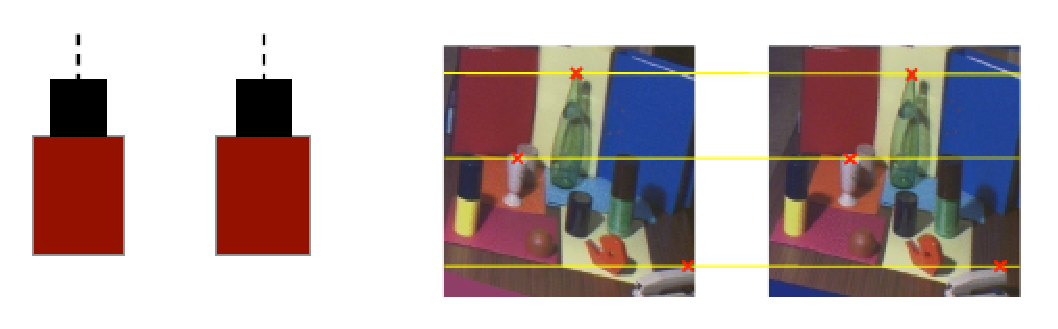
\includegraphics[width=0.7\textwidth]{images/cap2/VisionParalela.eps}
      \captionof{figure}{Visión paralela}
      \label{fig:VisionParalela}
  \end{minipage}

  \item \textbf{Visión cruzada:} las cámaras no están paralelas entre sí, tienen
  una inclinación de tal forma que el objetivo de cada cámara apunta hacia el
  lado contrario de una imagen. Por lo que los ejes ópticos se cruzan entre sí.
  Las líneas de correspondencia, también tienen sufren una inclinación.

  \begin{minipage}{\linewidth}
      \centering
      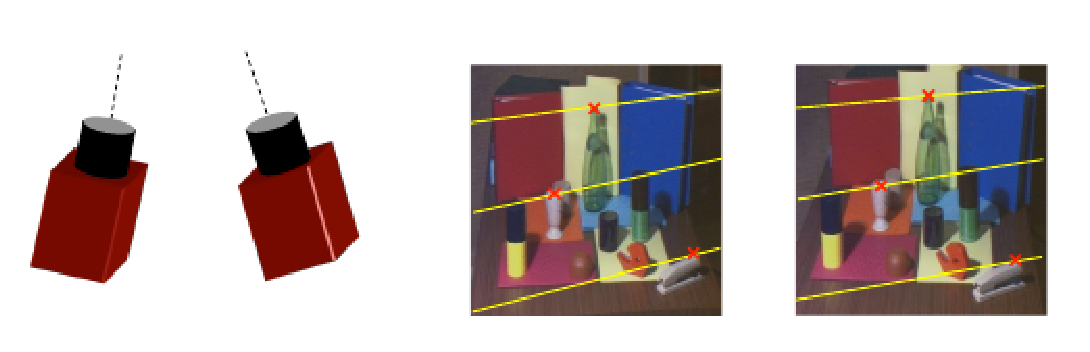
\includegraphics[width=0.7\textwidth]{images/cap2/VisionCruzada.eps}
      \captionof{figure}{Visión cruzada}
      \label{fig:VisionCruzada}
  \end{minipage}
\end{itemize}

% http://vfxio.com/PDFs/Parallel_vs_Converged.pdf
La visión cruzada tiene la desventaja de distorsionar las imágenes capturadas.
En la figura 2.4 se puede observar este efecto al fotografíar un muro de
ladrillos. Sin embargo, dependiendo del tipo de escena que se capture, esta
distorsión puede suponer un problema o no.

\begin{figure}[!th]
  \begin{center}
    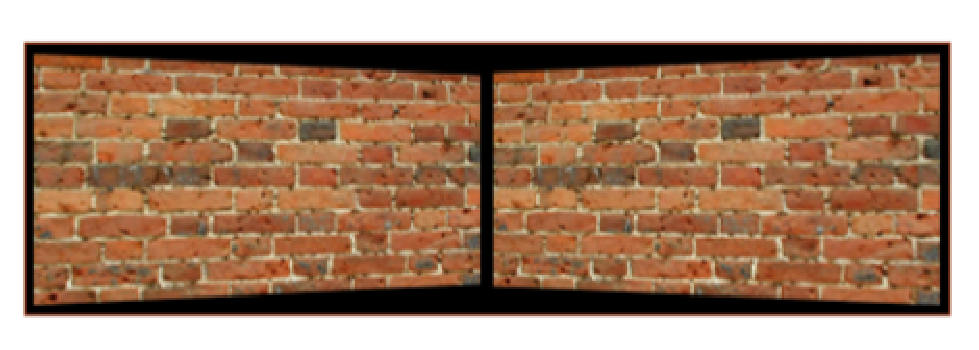
\includegraphics[width=0.5\textwidth]{images/cap2/VisionCruzadaMuro.eps}
    \caption{Muro distorsionado por visión cruzada}
    \label{fig:VisionCruzadaMuro}
  \end{center}
\end{figure}

La visión paralela por su parte, no distorsiona las imágenes capturadas, pero
también cuenta con otra serie de problemas. \textcolor{red}{Lorem ipsum dolor sit amet, consectetur adipisicing elit, sed do eiusmod tempor incididunt ut labore et dolore magna aliqua. Ut enim ad minim veniam, quis nostrud exercitation ullamco laboris nisi ut aliquip ex ea commodo consequat. Duis aute irure dolor in reprehenderit in voluptate velit esse cillum dolore eu fugiat nulla pariatur. Excepteur sint occaecat cupidatat non proident, sunt in culpa qui officia deserunt mollit anim id est laborum.}

%--------------------------------------
\subsection{Rectificación}
% https://en.wikipedia.org/wiki/Image_rectification

%--------------------------------------
\subsection{Disparidad}
% http://es.slideshare.net/RicardoSnchezCastill/vision-artificial-49264591
% http://stackoverflow.com/questions/17607312/difference-between-disparity-map-and-disparity-image-in-stereo-matching
% http://iie.fing.edu.uy/publicaciones/2005/Lec05a/Lec05a.pdf
La disparidad de dos imágenes establece la correspondencia entre los píxeles o
características que existen entre ambas para obtener la profundidad de la
escena. Conociendo la geometría del entorno y la cámara, de forma general, se
realiza una triangulación entre cada punto de las imágenes para obtener la
disparidad.

Metodos:


El objetivo final es poder construir una \textbf{imagen o mapa de disparidad}







% Disparidad....

% http://www.cesfelipesegundo.com/revista/articulos2011/Guerrero,%20J.M.pdf
% http://dmi.uib.es/~abasolo/cursorealidad/paco/Estereoscopia.html
%--------------------------------------
\subsection{Aplicaciones}
% https://www.ptgrey.com/tan/10570
La visión artificial resulta de gran utilidad en diferentes áreas de aplicación,
tanto en acciones repetitivas como peligrosas:

\begin{itemize}
  \item \textbf{Inspección y ensamblaje industrial:} el proyecto "Randon Bin
  Picking" (RBP) hace uso de visión estéreo para la búsqueda de piezas entre
  objetos de todo tipo para su rápida recuperación.
  % http://www.worldscientific.com/doi/suppl/10.1142/8766/suppl_file/8766_chap01.pdf
  \item \textbf{Apoyo en el diagnóstico médico:} en las últimas décadas la
  visión artificial se ha hecho un importante en la medicina para detectar,
  analizar y reconstruir la información obtenida.
  % http://www.ri.cmu.edu/pub_files/pub4/matthies_larry_2007_1/matthies_larry_2007_1.pdf
  \item \textbf{Exploración espacial:} en el proyecto de exploración Mars Rover
  (Mars Exploration Rover Mission) tiene como objetivo explorar la superficie
  de Marte en busca de rocas u otros elementos que prueben la existencia de
  agua.
  \item \textbf{Seguimiento (Tracking):} se hace uso en innumerables situaciones
  de carácter estadístico como contar el número o de en áreas de vigilancia y
  seguridad monitorizando trayectorias.
\end{itemize}


%+++++++++++++++++++++++++++++++++++++++++++++++++++++++++++++++++++++++++++++++
\section{Odometría}
\label{2:sec:3}

%--------------------------------------
\subsection{Mecánica}

%--------------------------------------
\subsection{Visual}


%+++++++++++++++++++++++++++++++++++++++++++++++++++++++++++++++++++++++++++++++
\section{Reconstrucción 3D}
\label{2:sec:4}


% http://slipguru.disi.unige.it/OLDslipguru/teaching/Vis2/LUCIDI/class5.pdf

% nube de puntos


%--------------------------------------
\subsection{SLAM}


%+++++++++++++++++++++++++++++++++++++++++++++++++++++++++++++++++++++++++++++++










%%%%%%%%%%%%%%%%%%%%%%%%%%%%%%%%%%%%%%%%%%%%%%%%%%%%%%%%%%%%%%%%%%%%%%%%%%%%%%%
\newpage{\pagestyle{empty}}
\thispagestyle{empty}

\chapter{Recursos y herramientas}
\label{chapter:recursos}

%%%%%%%%%%%%%%%%%%%%%%%%%%%%%%%%%%%%%%%%%%%%%%%%%%%%%%%%%%%%%%%%%%%%%%%%%%%%%%%
% Chapter 3: Recursos y herramientas
%%%%%%%%%%%%%%%%%%%%%%%%%%%%%%%%%%%%%%%%%%%%%%%%%%%%%%%%%%%%%%%%%%%%%%%%%%%%%%%

%++++++++++++++++++++++++++++++++++++++++++++++++++++++++++++++++++++++++++++++


Los capítulos intermedios servirán para cubrir los siguientes aspectos:
antecedentes, problemática o estado del arte, objetivos, fases y desarrollo del proyecto.

Bla, Bla, Bla, .....

%++++++++++++++++++++++++++++++++++++++++++++++++++++++++++++++++++++++++++++++
\section{Playstation Camera}
\label{3:sec1}

%++++++++++++++++++++++++++++++++++++++++++++++++++++++++++++++++++++++++++++++
\section{Silla}
\label{3:sec2}

%++++++++++++++++++++++++++++++++++++++++++++++++++++++++++++++++++++++++++++++
\section{ROS}
\label{3:sec3}


%%%%%%%%%%%%%%%%%%%%%%%%%%%%%%%%%%%%%%%%%%%%%%%%%%%%%%%%%%%%%%%%%%%%%%%%%%%%%%%

\chapter{Desarrollo}
\label{chapter:desarrollo}

%%%%%%%%%%%%%%%%%%%%%%%%%%%%%%%%%%%%%%%%%%%%%%%%%%%%%%%%%%%%%%%%%%%%%%%%%%%%%%%
% Chapter 4 : Desarrollo
%%%%%%%%%%%%%%%%%%%%%%%%%%%%%%%%%%%%%%%%%%%%%%%%%%%%%%%%%%%%%%%%%%%%%%%%%%%%%%%

%+++++++++++++++++++++++++++++++++++++++++++++++++++++++++++++++++++++++++++++++
Los capítulos intermedios servirán para cubrir los siguientes aspectos:
antecedentes, problemática o estado del arte, objetivos, fases y desarrollo del proyecto.
%+++++++++++++++++++++++++++++++++++++++++++++++++++++++++++++++++++++++++++++++

En el capítulo ~\ref{chapter:intro} se describió bla, bla, bla.....


%%%%%%%%%%%%%%%%%%%%%%%%%%%%%%%%%%%%%%%%%%%%%%%%%%%%%%%%%%%%%%%%%%%%%%%%%%%%%%%
\newpage{\pagestyle{empty}}
\thispagestyle{empty}

\chapter{Conclusiones y líneas futuras}
\label{chapter:conclusiones}

%%%%%%%%%%%%%%%%%%%%%%%%%%%%%%%%%%%%%%%%%%%%%%%%%%%%%%%%%%%%%%%%%%%%%%%%%%%%%
% Chapter 5: Conclusiones y Trabajos Futuros 
%%%%%%%%%%%%%%%%%%%%%%%%%%%%%%%%%%%%%%%%%%%%%%%%%%%%%%%%%%%%%%%%%%%%%%%%%%%%%%%

%+++++++++++++++++++++++++++++++++++++++++++++++++++++++++++++++++++++++++++++++
\section{Conclusiones}
\label{5:sec:1}
%%%%%%%%%%%%%%%%%%%%%%%%%%%%%%%%%%%%%%%%%%%%%%%%%%%%%%%%%%%%%%%%%%%%%%%%%%%%%
% Chapter 5: Conclusiones y Líneas Futuras 
%%%%%%%%%%%%%%%%%%%%%%%%%%%%%%%%%%%%%%%%%%%%%%%%%%%%%%%%%%%%%%%%%%%%%%%%%%%%%%%

%+++++++++++++++++++++++++++++++++++++++++++++++++++++++++++++++++++++++++++++++
% \section{Conclusiones}
% \label{5:sec:1}

En este trabajo se ha visto que las cámaras estereoscópicas permiten obtener
unas imágenes del mundo que le rodea muy próximas a la realidad. Por sí sola, la
odometría visual de este tipo de cámaras funciona muy bien en la mayoría de
situaciones, tanto en espacios cerrados como en lugares más abiertos, siendo un
claro competidor del sistema actual de la silla Perenquén, el uso de una cámara
RGB-D. Por otro lado, es importante mencionar que la integración de sensores
mecánicos y sensores láser permite corregir algunos de los problemas que son
propensos a ocurrir cuando las ocasiones lumínicas no son las idóneas.

Es necesario recordar, que es muy difícil recoger con exactitud la información
de la naturaleza, el entorno que nos rodea está vivo, sin embargo, la visión
estereoscópica sirve de pilar, junto con otros sensores para obtener la mayor
aproximación posible del mundo.

%+++++++++++++++++++++++++++++++++++++++++++++++++++++++++++++++++++++++++++++++


%+++++++++++++++++++++++++++++++++++++++++++++++++++++++++++++++++++++++++++++++
\section{Líneas futuras}
\label{5:sec:2}
%%%%%%%%%%%%%%%%%%%%%%%%%%%%%%%%%%%%%%%%%%%%%%%%%%%%%%%%%%%%%%%%%%%%%%%%%%%%%
% Chapter 5: Conclusiones y Líneas Futuras
%%%%%%%%%%%%%%%%%%%%%%%%%%%%%%%%%%%%%%%%%%%%%%%%%%%%%%%%%%%%%%%%%%%%%%%%%%%%%%%

%+++++++++++++++++++++++++++++++++++++++++++++++++++++++++++++++++++++++++++++++
% \section{Líneas futuras}
% \label{5:sec:2}

Más allá de la reconstrucción del mapa en 3D y la localización en el mismo, el
siguiente punto más atractivo es la detección y posterior esquiva de los
obstáculos en el camino del robot. Con este objetivo cumplido, el robot podría
navegar de forma autónoma.

Por otro lado, en función de los buenos resultados con la visión estéreo, se
debería analizar que otros sistemas alternativos a PlayStation Camera existen.

%+++++++++++++++++++++++++++++++++++++++++++++++++++++++++++++++++++++++++++++++


%+++++++++++++++++++++++++++++++++++++++++++++++++++++++++++++++++++++++++++++++


%%%%%%%%%%%%%%%%%%%%%%%%%%%%%%%%%%%%%%%%%%%%%%%%%%%%%%%%%%%%%%%%%%%%%%%%%%%%%%%
\newpage{\pagestyle{empty}}
\thispagestyle{empty}

\chapter{Summary and Conclusions }
\label{chapter:summary}

%%%%%%%%%%%%%%%%%%%%%%%%%%%%%%%%%%%%%%%%%%%%%%%%%%%%%%%%%%%%%%%%%%%%%%%%%%%%%
% Chapter 6: Conclusions and future work lines
%%%%%%%%%%%%%%%%%%%%%%%%%%%%%%%%%%%%%%%%%%%%%%%%%%%%%%%%%%%%%%%%%%%%%%%%%%%%%%%

%+++++++++++++++++++++++++++++++++++++++++++++++++++++++++++++++++++++++++++++++
\section{Conclusions}
\label{6:sec:1}
%%%%%%%%%%%%%%%%%%%%%%%%%%%%%%%%%%%%%%%%%%%%%%%%%%%%%%%%%%%%%%%%%%%%%%%%%%%%%
% Chapter 6: Conclusions and future work lines
%%%%%%%%%%%%%%%%%%%%%%%%%%%%%%%%%%%%%%%%%%%%%%%%%%%%%%%%%%%%%%%%%%%%%%%%%%%%%%%

%+++++++++++++++++++++++++++++++++++++++++++++++++++++++++++++++++++++++++++++++
% \section{Conclusions}
% \label{6:sec:1}

In this project we have seen that stereoscopic cameras allow to obtain images of
the world very close to reality. Use only visual odometry of these cameras works
fine in most situations both indoors and in more open places, being a clear
competitor to the current system of the Perenquén project, using a camera RGB-D.
Furthermore, it is important to mention that the integration of mechanical
sensors and laser sensors allow to correct some of the problems that are likely
to happen when the lighting conditions are not ideal.

It is need to remember, it is very difficult to collect accurate information
from nature, the environment around us is alive, however, stereo vision is the
key, along with other sensors to obtain the best possible approach of the world.

%+++++++++++++++++++++++++++++++++++++++++++++++++++++++++++++++++++++++++++++++


%+++++++++++++++++++++++++++++++++++++++++++++++++++++++++++++++++++++++++++++++
\section{Future work lines}
\label{6:sec:2}
%%%%%%%%%%%%%%%%%%%%%%%%%%%%%%%%%%%%%%%%%%%%%%%%%%%%%%%%%%%%%%%%%%%%%%%%%%%%%
% Chapter 6: Conclusions and future work lines
%%%%%%%%%%%%%%%%%%%%%%%%%%%%%%%%%%%%%%%%%%%%%%%%%%%%%%%%%%%%%%%%%%%%%%%%%%%%%%%

%+++++++++++++++++++++++++++++++++++++++++++++++++++++++++++++++++++++++++++++++
% \section{Future work lines}
% \label{6:sec:2}

Beyond 3D mapping and localization in the map, the next most attractive point is
the detection and subsequent dodging of obstacles in the path of the robot. With
this goal achieved, the robot could navigate autonomously.

Furthermore, according to good results with stereo vision, it should analyze
other existing alternative systems PlayStation Camera.

%+++++++++++++++++++++++++++++++++++++++++++++++++++++++++++++++++++++++++++++++


%+++++++++++++++++++++++++++++++++++++++++++++++++++++++++++++++++++++++++++++++




%%%%%%%%%%%%%%%%%%%%%%%%%%%%%%%%%%%%%%%%%%%%%%%%%%%%%%%%%%%%%%%%%%%%%%%%%%%%%%%
\newpage{\pagestyle{empty}}
\thispagestyle{empty}

\chapter{Presupuesto}
\label{chapter:presupuesto}

%%%%%%%%%%%%%%%%%%%%%%%%%%%%%%%%%%%%%%%%%%%%%%%%%%%%%%%%%%%%%%%%%%%%%%%%%%%%%
% Chapter 7: Presupuesto
%%%%%%%%%%%%%%%%%%%%%%%%%%%%%%%%%%%%%%%%%%%%%%%%%%%%%%%%%%%%%%%%%%%%%%%%%%%%%%%

%+++++++++++++++++++++++++++++++++++++++++++++++++++++++++++++++++++++++++++++++
\section{Presupuesto total}
\label{7:sec:1}


%--------------------------------------------------------------------------
\begin{table}[!ht]
\begin{center}
\begin{tabular}{|p{80mm}|p{40mm}|} \hline 
\textbf{Elemento } & \textbf{Precio} \\ \hline
PlayStation Camera &
\euro{59.95}
\\
\hline

\end{tabular}
\end{center}
\caption{Material}
\label{table:material}
\end{table}

%--------------------------------------

\begin{table}[!ht]
\begin{center}
\begin{tabular}{|p{80mm}|p{20mm}|p{20mm}||p{20mm}|} \hline 
\textbf{Tarea} & \textbf{Horas} & \textbf{Precio} & \textbf{Total} \\ \hline
Investigación &
80h &
\euro{15} &
\euro{1200}
\\
\hline

Implementación &
120h &
\euro{20} &
\euro{2400}
\\
\hline

Escritura de la Memoria &
40h &
\euro{5} &
\euro{200}
\\
\hline

&
&
&
\euro{3800}
\\
\hline

\end{tabular}
\end{center}
\caption{Tareas}
\label{table:horas}
\end{table}

%--------------------------------------

\begin{table}[!ht]
\begin{center}
\begin{tabular}{|p{80mm}|p{40mm}|} \hline 
\textbf{Elemento } & \textbf{Precio} \\ \hline
Material &
\euro{59.95}
\\
\hline

Tareas &
\euro{3800}
\\
\hline

&
\euro{3859.95}
\\
\hline

\end{tabular}
\end{center}
\caption{Presupuesto total}
\label{table:presupuesto}
\end{table}


%+++++++++++++++++++++++++++++++++++++++++++++++++++++++++++++++++++++++++++++++


%%%%%%%%%%%%%%%%%%%%%%%%%%%%%%%%%%%%%%%%%%%%%%%%%%%%%%%%%%%%%%%%%%%%%%%%%%%%%%%

%%%%%%%%%%%%%%%%%%%%%%%%%%%%%%%%%%%%%%%%%%%%%%%%%%%%%%%%%%%%%%%%%%%%%%%%%%%%%%%
\newpage{\pagestyle{empty}}
\thispagestyle{empty}
\begin{appendix}

\chapter{Launchs}
\label{appendix:1}
%%%%%%%%%%%%%%%%%%%%%%%%%%%%%%%%%%%%%%%%%%%%%%%%%%%%%%%%%%%%%%%%%%%%%%%%%%%%%%%
% Apéndice: Launchs
%%%%%%%%%%%%%%%%%%%%%%%%%%%%%%%%%%%%%%%%%%%%%%%%%%%%%%%%%%%%%%%%%%%%%%%%%%%%%%%

%++++++++++++++++++++++++++++++++++++++++++++++++++++++++++++++++++++++++++++++
\section{Launch: PlayStation Camera en Carro}
\label{appendix:carrito}
\input{appendix/launchs/carrito.tex}

%++++++++++++++++++++++++++++++++++++++++++++++++++++++++++++++++++++++++++++++


% \chapter{Título del Apéndice 1}
% \label{appendix:1}
% \input{appendix/apendice1.tex}
% 
% \chapter{Título del Apéndice 2}
% \label{appendix:2}
% \input{appendix/apendice2.tex}

\end{appendix}

%%%%%%%%%%%%%%%%%%%%%%%%%%%%%%%%%%%%%%%%%%%%%%%%%%%%%%%%%%%%%%%%%%%%%%%%%%%%%%%
\addcontentsline{toc}{chapter}{Bibliografía}
\bibliographystyle{plain}

\bibliography{memtfg}
\nocite{*}

%%%%%%%%%%%%%%%%%%%%%%%%%%%%%%%%%%%%%%%%%%%%%%%%%%%%%%%%%%%%%%%%%%%%%%%%%%%%%%%

\end{document}
